% $ based on Id: sample_english-v1.2.tex,v 1.2 2007/04/12 21:05:22 zlb Exp $
% $Id: sample_english.tex 6 2011-01-24 13:13:33Z hsqi $

\documentclass[english]{cccconf}
%\documentclass[usemulticol,english]{cccconf}
\usepackage[comma,numbers,square,sort&compress]{natbib}
\usepackage{epstopdf}
\usepackage{comment}
\usepackage{subcaption}
\usepackage{color}
\usepackage{lipsum}
\usepackage{multicol}
\usepackage{amssymb}
\usepackage{amsmath}
\usepackage{bm}
\usepackage{amsfonts}
\usepackage{multirow}
\usepackage{graphicx}
\usepackage{mathtools, amssymb}
\usepackage[comma,numbers,square,sort&compress]{natbib}
\usepackage{CJK}
\usepackage{graphicx}
\usepackage{epsfig}
\usepackage{float}
\usepackage{multirow}
\usepackage{algorithm}
\usepackage{algorithmic}
\usepackage{indentfirst}
\usepackage{booktabs}
\usepackage{amsmath}



\begin{document}

\title{Competition of Social Opinions on Two Layer Networks}

% Note: the first argument in the \affiliation command is optional.
% It defines a label for the affiliation which can be used in the \aref
% command. If there is only one affiliation for all authors, then the
% optional argument in the \affiliation command should be suppressed,
% and the \aref command should also be removed after each author in
% \author command, in this case the affiliation will not be numbered.
% \author{First Author, Second Author, Third Author}
% \affiliation{Chinese Academy of Sciences, Beijing 100190, P.~R.~China\email{ccc@amss.ac.cn}}

\author{Cho Hyunchel \aref{amss,hit},
        A. Mahmood \aref{amss,hit},
        Lin Wang \aref{amss,hit}}
\affiliation[amss]{Department of Automation, Shanghai Jiao Tong University, Shanghai 200240, P.~R.~China}
\affiliation[hit]{Key Laboratory of System Control and Information Processing, Ministry of Education of China, Shanghai 200240, P.~R.~China
        \email{leighsix@naver.com}\email{arfan499@sjtu.edu.cn}\email{wanglin@sjtu.edu.cn}}

\maketitle

\begin{abstract}
Social conflict usually can be investigated based on competition on two-layers network. In this paper, a competition model is studied on interconnected networks with two-layer opinions, where the first layer is opinion formation and the second layer is decision making. Starting with a polarized competition case where layer A has all positive opinion and layer B has all negative opinion, competition simulations are considered based on different network structures. Various simulations are implemented with different structural models, that are created by changing network structure and the number of edges and nodes. Specifically, consensus part of models are estimated with simulation results. Through the estimation of consensus, it is found out that internal edges have the tendency to keep and maintain the state of each layer, and  external edges not only help to make consensus of two layers, but there are also efficient numbers of external edge for making consensus. Our results indicate that interconnected networks can have more probability for social consensus by changing and controlling the number of internal and external edges.  

\end{abstract}

\keywords{Interconnected Networks, Opinion Dynamics, Decision Making}

% Please remove or comment out the following line if the footnote is not necessary
\footnotetext{This work was supported by the National Natural Science Foundation of China under Grant Nos 61873167, 61473189, the Natural Science Foundation of Shanghai (No.17ZR1445200).}

\section{Introduction}
In various situations ranging from voting to adoption of new policies, it is widely recognized that opinion formation and decision making formation have mutual interaction as interconnected networks\cite{bianconi2018,domenico2013,tomasini2015, kimsangwoo2012,newman2010,boccaletti2014,mikko2013,huberman2004}. Many researchers have devoted to modeling and analyzing competition on opinion dynamics\cite{amato2017,quattrociocchi2014,haibo2017, hua2014}, voter model\cite{redner2017}, game theory\cite{smyrnakis2019} and many more\cite{danziger2019,namkhanhvu2017,laguna2004,masuda2015,zuev2012, shenyu2018}.  
 
For competition of interconnected networks, many researches have been performed in the various networks, for example the dissemination of computer viruses, messages, opinions, memes, diseases and rumors\cite{bianconi2018,hua2014,shenyu2018,alvarez2016,gomez2015,diep2017,rocca2014,velasquez2018}. Opinion dynamics on two-layer or multilayer networks are investigated, based on \textit{Abrams-Strogatz(AS)} model\cite{abrams2003,vazquez2010} and $M$ model\cite{rocca2014}. It has been focused on that under what conditions all agents reach a consensus or dissent. As the result of pre-existed research, it has been proved that the system can make positive consensus, negative consensus or coexistence parts in interconnected competition of the social network under the certain range of volatility, reinforcement, or prestige. Also, the threshold or critical point for transition are found out to explain and analyze the social phenomena in real world such as the legislation, election result, and social network\cite{alvarez2016, amato2017, diep2017}. In \cite{gomez2015}, it is shown that the transition from localized to mixed status occurs via a cascade from poorly connected nodes in layers to those highly connected ones. In addition, the main features, such as transition and cascade, found in Monte Carlo simulation is exactly characterized by the mean-field theory and magnetization\cite{alvarez2016, diep2017, amato2017, gomez2015}.   

In this paper, we investigate the competitions on two interconnected networks with various different structures, considering which structure have more probability consensus results. With Monte Carlos simulations, consensus of interconnected networks would be estimated and compared with the other models. MC simulations show the vital influence of internal and external degree with theses results that the larger the average internal degrees of one layer is, the more the tendency to keep and maintain the state of the layer is, and that external degree helps to make social consensus. Finally, We would provide three conditions that can help to make social consensus. This paper gives some solutions to find the network structures that make efficient consensus of two layers. In real world, it could be used as a tool for analyzing legislation problems, making efficient decision-making system and solving the social conflict.  

The paper is organized as follows. In section 2, competition dynamics of interconnected network, that is applied to each layer, are described. In section 3, the simulation results of different structural networks are presented. Finally, in section 4, the simulation results will be summarized.

\section{Modeling}
The model consists of two layers, and each layer has different dynamics. For layer A, the node change its states according to $M$ model as introduced in \cite{rocca2014}. Here, we choose $M=2$, that each node has four states $(-2, -1, +1, +2)$. For each link $(k, j)$ belong to layer A,  the dynamics are designed as follows:
\begin{itemize}
\item Compromise : if they have opposite orientations, their states become more moderate with probability $q$ :

\begin{align*}
\mbox{if } S_k<0 \mbox{ and } S_j>0  \Rightarrow (S_k, S_j) \rightarrow (S_k^r, S_j^l) \mbox{ with } prob.q,\\
\mbox{if } S_k>0 \mbox{ and } S_j<0  \Rightarrow (S_k, S_j) \rightarrow (S_k^l, S_j^r) \mbox{ with } prob.q.
\end{align*}
If $S_k = \pm1$ and $S_j = \mp1$, one switches orientation at random:
\begin{align*}
(\pm 1, \mp 1)\rightarrow \left\{\begin{matrix}
(+1, +1) \mbox{ with } prob.q/2,
\\(-1, -1)\mbox{ with } prob.q/2.
\end{matrix}\right.
\end{align*}
\item Persuasion : if they have the same orientation, their states become more extreme with probability $p$ :
\begin{align*}
\mbox{if } S_k<0 \mbox{ and } S_j<0  \Rightarrow (S_k, S_j) \rightarrow (S_k^l, S_j^l) \mbox{ with } prob.p,\\
\mbox{if } S_k>0 \mbox{ and } S_j>0  \Rightarrow (S_k, S_j) \rightarrow (S_k^r, S_j^r) \mbox{ with } prob.p.
\end{align*}
\end{itemize}
For each external link $(k,j)$ with $k$ belong to layer A, the state of node $k$ is updated according to :
\begin{itemize}
\item $S_k \times S_j < 0$ :
\begin{align*}
\mbox{if } S_k<0 \mbox{ and } S_j>0  \Rightarrow (S_k, S_j) \rightarrow (S_k^r, S_j) \mbox{ with } prob.q,\\
\mbox{if } S_k>0 \mbox{ and } S_j<0  \Rightarrow (S_k, S_j) \rightarrow (S_k^l, S_j) \mbox{ with } prob.q.
\end{align*}
\item $S_k \times S_j > 0$ :
\begin{align*}
\mbox{if } S_k<0 \mbox{ and } S_j<0  \Rightarrow (S_k, S_j) \rightarrow (S_k^l, S_j) \mbox{ with } prob.p,\\
\mbox{if } S_k>0 \mbox{ and } S_j>0  \Rightarrow (S_k, S_j) \rightarrow (S_k^r, S_j) \mbox{ with } prob.p.
\end{align*}
\end{itemize}
Here, $S_k^r$ and $S_k^l$ denote the right and left neighboring states of $k$, defined as
\begin{align*}
S_k^r &= \left\{\begin{matrix}
1,\mbox{ for } S_k= -1
\\ M,\mbox{ for } S_k=M
\\ S_k + 1,\mbox{ otherwise }, 
\end{matrix}\right. &
S_k^l &= \left\{\begin{matrix}
-1,\mbox{ for } S_k= 1
\\ -M,\mbox{ for } S_k=-M
\\ S_k - 1,\mbox{ otherwise }.
\end{matrix}\right.
\end{align*}


The sign of $S^A$ represents its opinion orientation and its absolute value $|S^A|$ measures the intensity of its opinion. So, $|S^A|=2$ represents to a positive or a negative extremist, while  $|S^A|=1$ correspond to a moderate opinion of each side. In case of internal link $(k, j)$ belong to layer A, if the nodes are the same orientation$(S_kS_j>0)$, then with probability $p$ the states of nodes become extreme$(S_k=\pm1 \rightarrow \pm2, S_j= \pm1 \rightarrow \pm2)$ if they are moderate, or remain extreme if they are already extreme$(S_k=\pm2 \rightarrow \pm2, S_j= \pm2 \rightarrow \pm2)$. Inversely if the nodes are opposite orientations$(S_kS_j<0)$, with probability $q$ the states of nodes become moderate it they are extreme$(S_k=\pm2 \rightarrow \pm1, S_j= \pm2 \rightarrow \pm1)$, or switch orientations if they are already moderate$(S_k=\pm1 \rightarrow \mp1, S_j= \pm1 \rightarrow \mp1)$.  In case of interaction between layer A node and layer B node, layer A node follows opinion dynamics formula, but the state of layer B node does not change. In other words, the state of layer B affects layer A, but this dynamics does not affect state of layer B node. For example, one of layer A node, $S_k = +2$ is connected with one of layer B node, $S_j = -1$. In this case, $S_k$ will change into $S_k = +1$ with $prob.q$. But $S_j$ will not change, which indicates that the states of layer B will influence the states of layer A.

The dynamics of layer B follows the decision-making dynamics as introduced in \cite{abrams2003, vazquez2010}. The state of node i in layer B can be +1 and -1, and it updates according to

\begin{equation}
P_B(S_i \rightarrow -S_i)= \left \{\frac{n^{-S_i}}{i_i + e_i}\right \}^\beta,
\end{equation}

where $i_i$ is the number of internal edges and $e_i$ is the number of external edges. $n^{-S_i}$ is the number of neighbors of i with opposite state $-S_i$. $\beta(\geq 0)$ is the volatility exponent that measures how prone a node change its state. If $\beta \simeq 0$, a node is very likely to change its state. Inversely, if $\beta \gg 1$, a node is unlikely to change its state. Also, this formula means that the more the nodes are connected with the opposite state, the easier the nodes can change into the opposite state.
The states of nodes in layer B can be $+1$ and $-1$. \\
\begin{figure}[!htb]
  \centering
  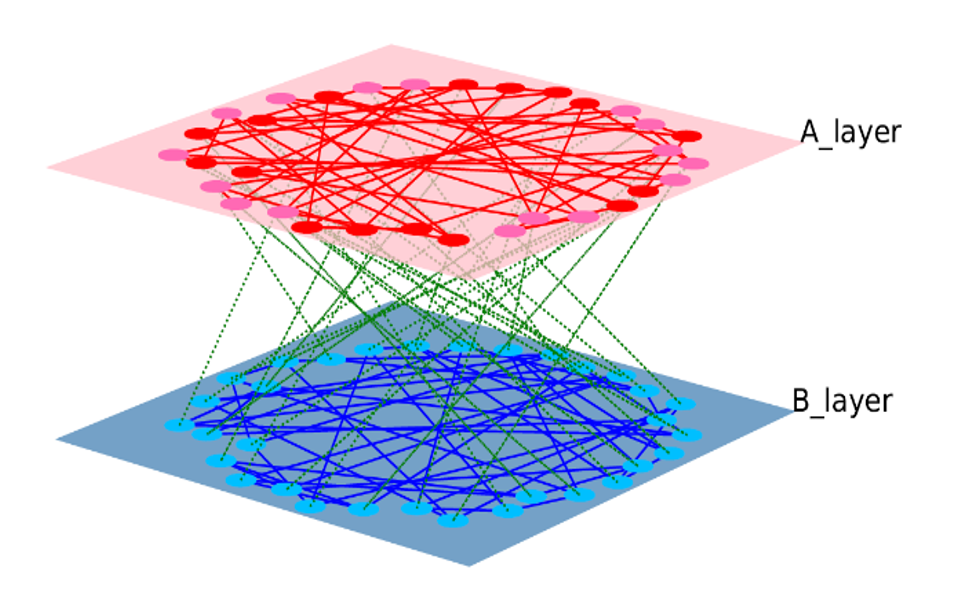
\includegraphics[width=\hsize]{FIG1.png}
  \caption{Competition of Interconnected Network}
  \label{Fig1}
\end{figure}


\section{Simulations and Analysis}
To start with a polarized competition, as the initial conditions,  nodes in layer A are all positive, and nodes in layer B are all negative. As nodes in layer A can be various states, it begins with the status where an half of nodes are $+1$ and the others are $+2$. And the nodes of layer B have only $-1$. 

There are two parameters in the dynamics of layer A. To simply represent the probability $p$ and probability $q$ together, we set $\gamma = p/q$ based on $p+q=1$. Here, $\gamma$ represents the tendency of opinion such as extreme or moderate, which is scaled to be 0 to 2. However, the scale of $\beta$, in the dynamics of layer B, depends on the total number of degrees. 

To implement the interconnected dynamics, one step consists of two layers dynamics, where for every link with at least one node in layer A will be checked, and every node in layer B will updates its state according to the decision-making dynamics. Each simulation takes 30 steps, and 100 simulations are considered  for each set of parameters. And we use \textit{`Average State'(AS)} to measure two layer state.

\begin{equation}
AS = avg\left( {\sum\limits_i^{{K^A}} {S_i^A/4} } \right) + avg\left( {\sum\limits_i^{{K^B}} {S_i^B/2} } \right).
\end{equation}

With \textit{AS}, it could be checked whether the consensus happens or not in accordance with $\gamma$ and $\beta$ changing.  If the positive consensus happens, it would be close to the value of $+1$ and if the negative consensus happens, it would be close to the value of $-1$. The values between $+1$ and $-1$ are not on the consensus yet, so these states are considered as belonging to the coexistence part.

\begin{figure*}[!htb]
	\centering
	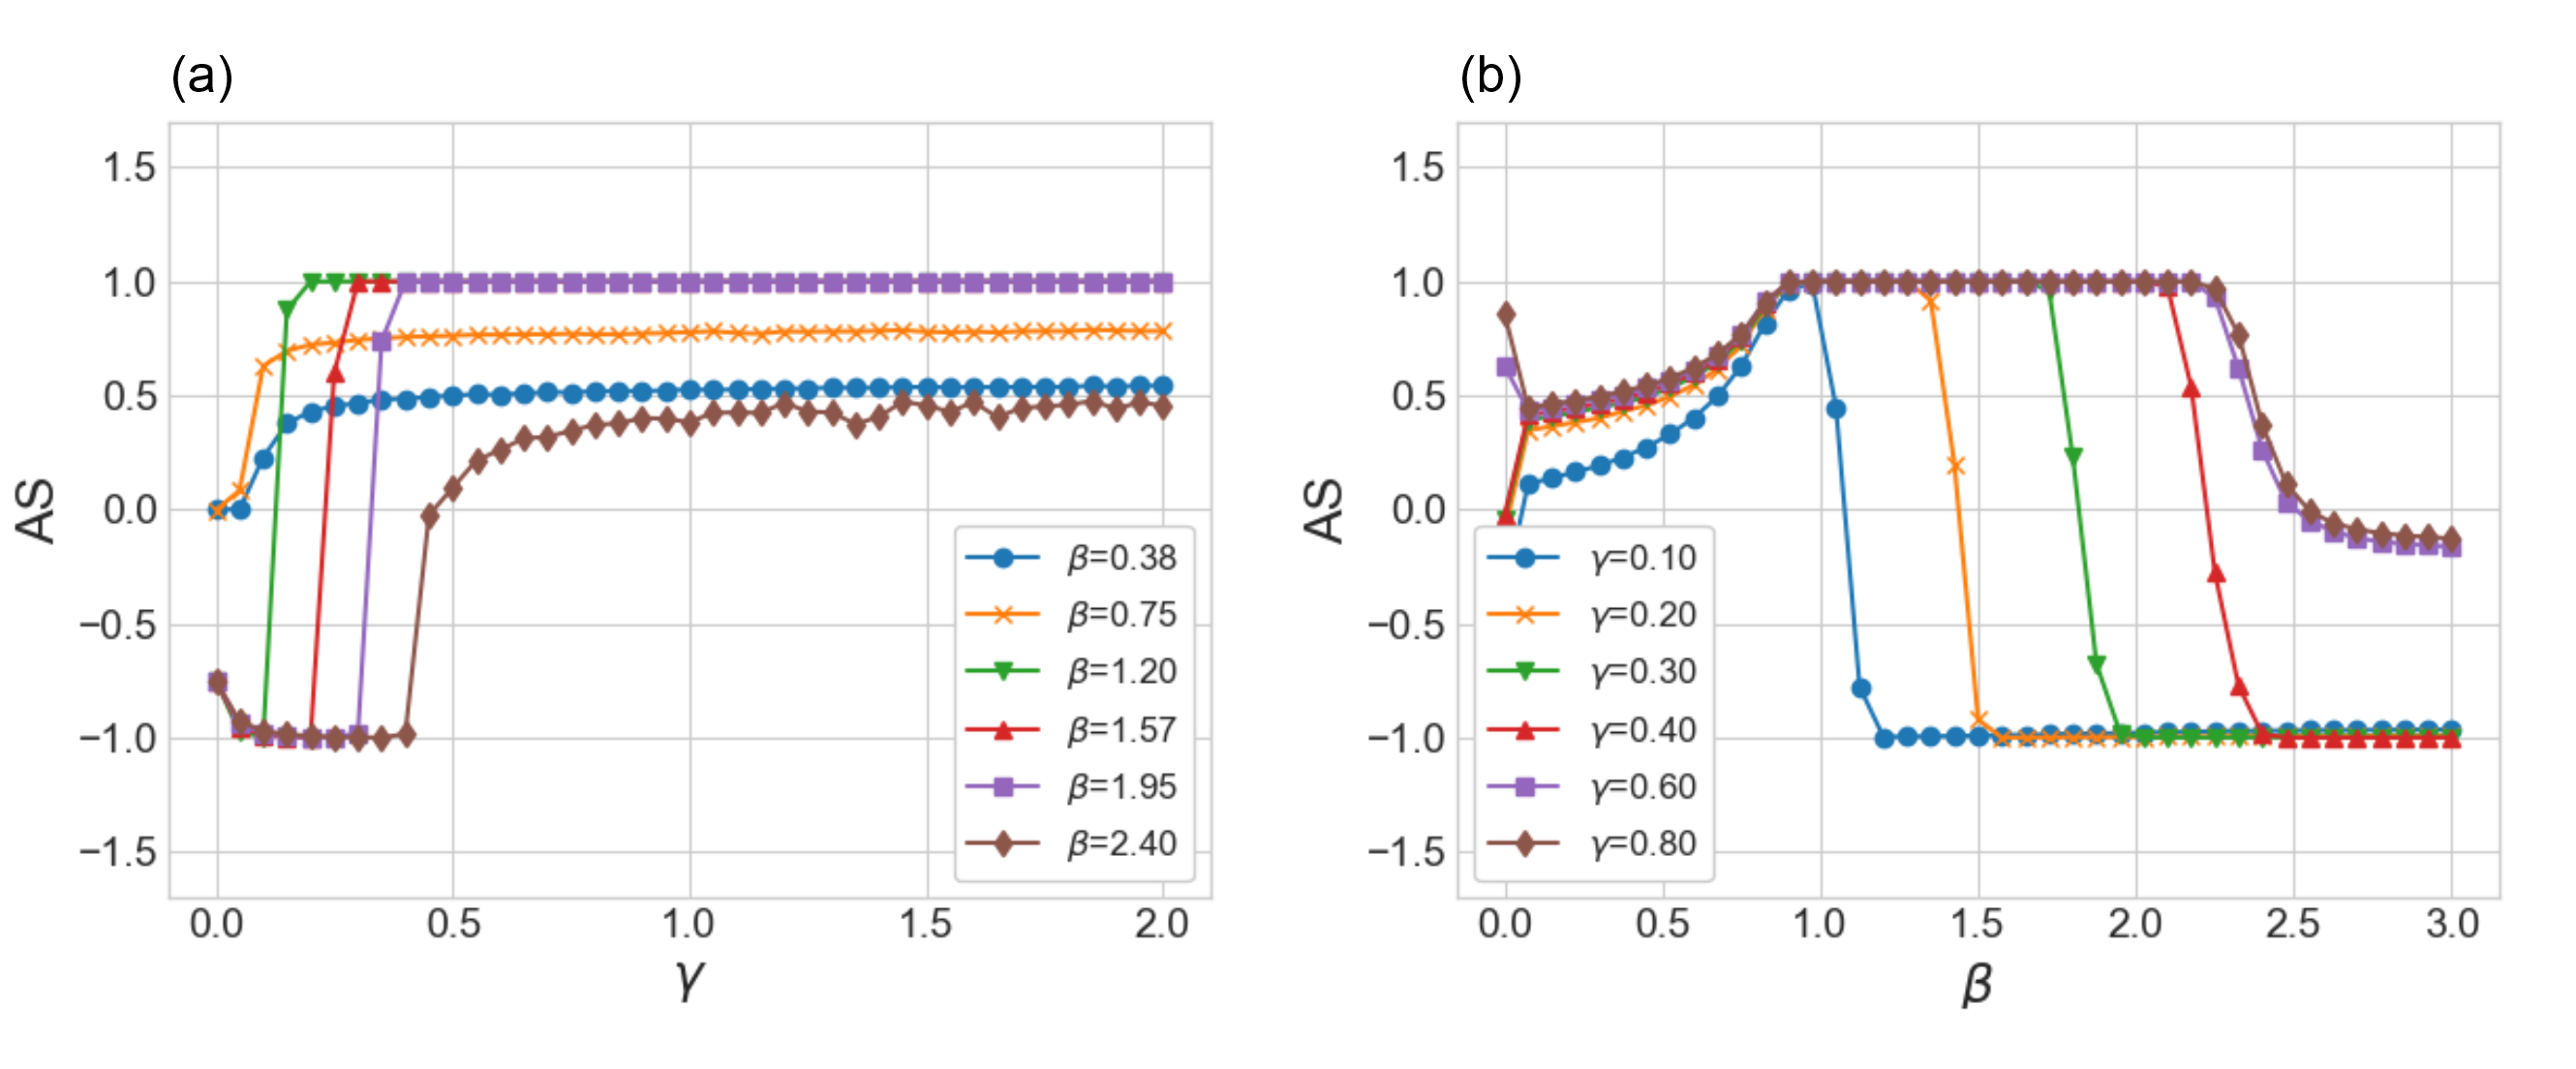
\includegraphics[width=\hsize]{FIG2.png}
	\caption{(a) $\gamma$-\textit{AS} chart according to certain $\beta$ values. (b) $\beta$-\textit{AS} chart according to certain $\gamma$ values.}
	\label{Fig2}
\end{figure*}

To estimate and evaluate consensus results of network structures according to all $\gamma$s and all $\beta$s, we use and compute $4$ kinds of measures including \textit{`AS total'}, \textit{`Positive Consensus Ratio'(PCR)}, \textit{`Negative Consensus ratio'(NCR)}, \textit{`Consensus Ratio'(CR)}. \textit{AS total} means the summation of \textit{AS} for all $\gamma$s and all $\beta$s. In eqs(3), ${A{S_{{\gamma _i},{\beta _j}}}}$ means $AS$ value with parameters, $\gamma_i$ and $\beta_j$. It shows the total orientation and intensity of networks. \textit{PCR} is the ratio of positive consensus in the simulation result. When ${A{S_{{\gamma _i},{\beta _j}}} \simeq  1}$, it is considered as positive consensus. So the number is counted, and ratio of the counted number is calculated as \textit{PCR}. And \textit{NCR} is the ratio of negative consensus part in the simulation result. It is the same calculated way with \text{PCR}, when ${A{S_{{\gamma _i},{\beta _j}}} \simeq  -1}$. \textit{CR} is the ratio of consensus part in the simulation result, summation of \textit{PCR} and \textit{NCR}.

\begin{equation}
\begin{array}{cl}
AS\mbox{ \textit{total} } = \frac{{\sum\limits_j^m {\sum\limits_i^n {A{S_{{\gamma _i},{\beta _j}}}} } }}{{n \times m }}, &
\begin{array}{l}
\gamma  = \left\{ {{\gamma _{\rm{1}}},{\gamma _{\rm{2}}},\left. {\cdot\cdot\cdot,{\gamma _n}} \right\}} \right.\\
\beta {\rm{ = }}\left\{ {{\beta _{\rm{1}}},{\beta _{\rm{2}}},\left. {\cdot\cdot\cdot,{\beta _m}} \right\}} \right.
\end{array}.\
\end{array}
\end{equation}

\begin{equation}
PCR = \frac{{\sum\limits_j^m {\sum\limits_i^n {(A{S_{{\gamma _i},{\beta _j}}} \simeq  1 \to 1)} } }}{{n \times m}}.
\end{equation}

\begin{equation}
NCR = \frac{{\sum\limits_j^m {\sum\limits_i^n {(A{S_{{\gamma _i},{\beta _j}}} \simeq   - 1 \to 1)} } }}{{n \times m}}.
\end{equation}

\subsection{Competition on Random Regular Networks}
For the first simulation, each layer consists of random regular network that has $N$ nodes with $k$ internal edges\cite{kimsangwoo2012, bela2001}. Each node of a layer is connected with a random node on the other layer. That means all the node has only 1 external un-directed edge. Basically, the simulations are done with $N=2048$, and $k=5$. 

The simulation results are shown in Fig.~\ref{Fig2} and Fig.~\ref{Fig3}. Fig.~\ref{Fig2}(a) shows that when $\gamma$ increases, if $\beta$ is in some range$(1.2 < \beta < 1.95)$, it normally tends to make positive consensus. But, if $\beta$ is too low or too large, it cannot make consensus.
In Fig.~\ref{Fig2}(b), as $\beta$ increases, it normally tends to make positive or negative consensus. But, when $\gamma$ is very low($\gamma \le 0.1$), it cannot make positive consensus. On the other hand, when $\gamma$ is large enough, it can make positive consensus. But, $\beta$ is large enough, it can change into negative consensus. When both of $\gamma$ and $\beta$ are large enough, its state is in the coexistence part. 
\begin{figure}[!htb]
	\centering
	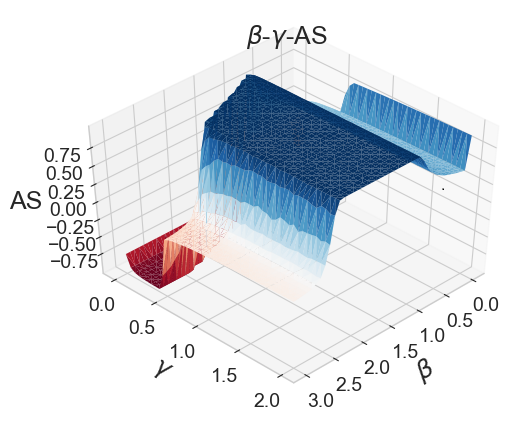
\includegraphics[width=\hsize]{FIG3.png}
	\caption{Random Regular  Networks result : \textit{AS} with changing $\gamma$ and $\beta$}
	\label{Fig3}
\end{figure}
\begin{figure*}[!htb]
	\centering
	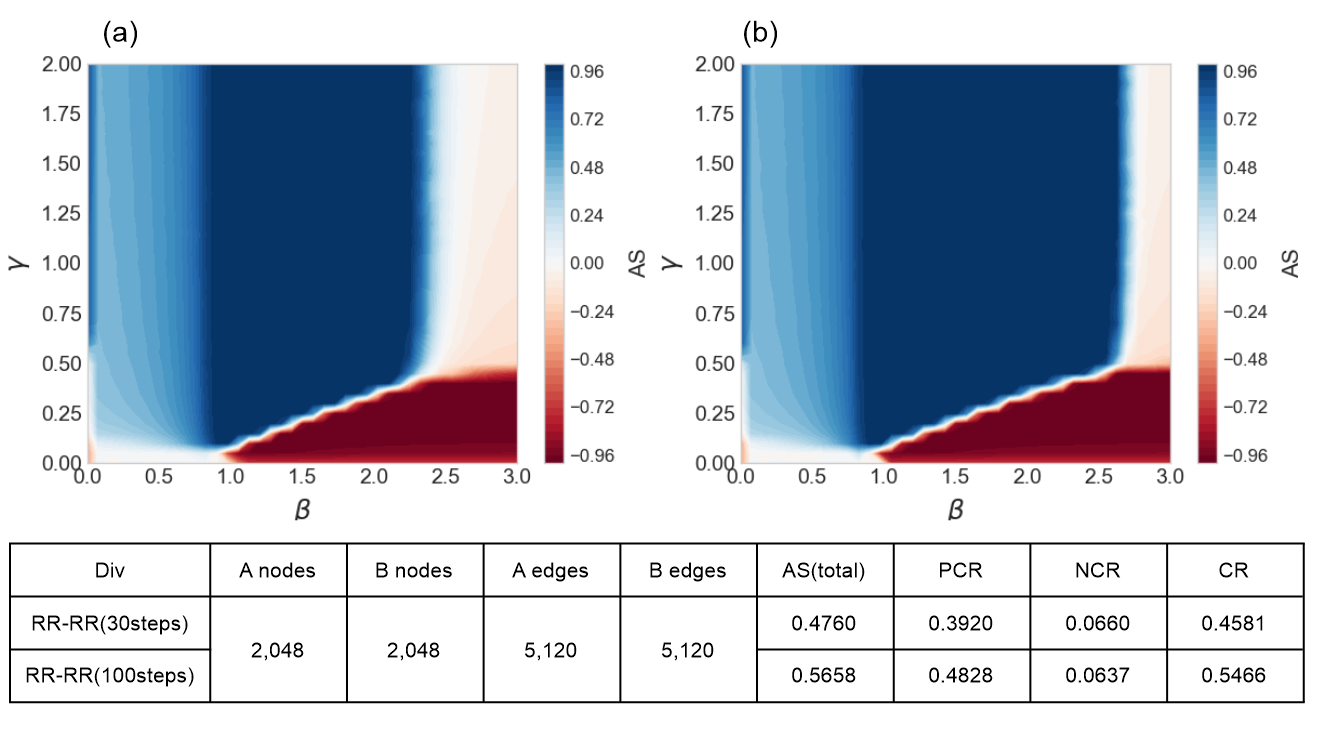
\includegraphics[width=\hsize]{FIG4.png}
	\caption{Comparison between 30 steps dynamics result and 100 steps dynamics result}
	\label{Fig4}
\end{figure*}
In Fig.~\ref{Fig3}, that shows the states of two layers according to all $\gamma$s and all $\beta$s. The $X$-axis is the $\gamma$ and the $Y$-axis is the $\beta$, and the $Z$-axis represents \textit{AS}. The closer the color is to be blue, the more it has positive consensus. And the closer the color is to be red, the more it has negative consensus. A light and white areas have coexistence with positive states and negative states mixed. This chart has two areas for coexistence, when $\beta$ is very low or high. Which means, when $\beta$ is in some range, interconnected network can make positive or negative consensus with $\gamma$ value.     

With this simulation, the dynamics steps are increased from $30$ steps to $100$ steps. Consensus and two layer states are estimated as \textit{AS total}, \textit{CR}, \textit{PCR}, and \textit{NCR}. Fig.~\ref{Fig4} provides the comparison between $30$ steps and $100$ steps dynamics with simulation properties. In Fig.4 table, \textit{AS total}, \textit{CR} and \textit{PCR} of 100 steps dynamics  has larger than $30$ steps dynamics. As the dynamics steps are increased, the layer states are more stable and positive consensus happens increasingly. It is analyzed that social opinion is likely to achieve the consensus if it was given enough time with stable reinforcement($\gamma$) above critical point.

\subsection{Competition on Networks with different number of external links}
\begin{figure}[!htb]
	\centering
	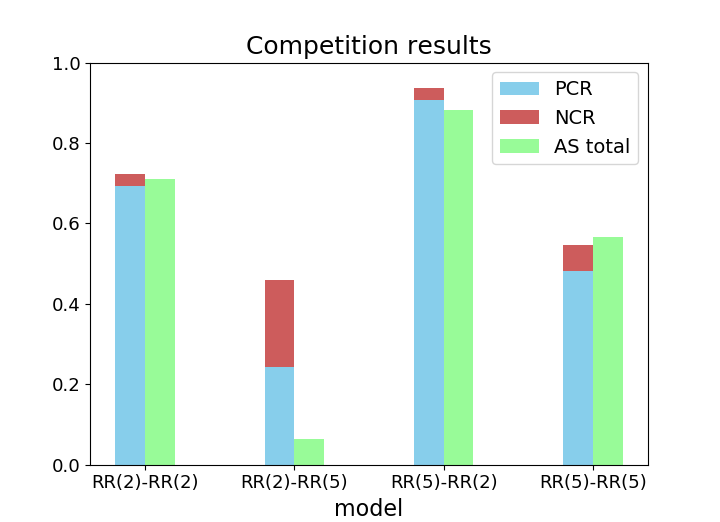
\includegraphics[width=\hsize]{FIG5.png}
	\caption{Leader Model results(\textit{LM(n)} : Leader Model where the number of layer B nodes are reduced by $1/n$)}
	\label{Fig5}
\end{figure}
The models, which would be called as Leader Model, are the redesigned model where the number of layer B nodes is reduced at certain rate such as $1/16$ or $1/4$, and increase the number of external edges in layer B by certain rate like $16$ times or $4$ times. In other words, each layer A node has one external edge, but each layer B node has $16$ or $4$ external edges. That is, as social network relation, it can be analyzed that one node of layer B represents the nodes of layer A. $\gamma$ scale is same as the Random Regular Networks Model. But, $\beta$ scale depends on the number of degrees. So the $\beta$ scale is adjusted to same values as the Random Regular Networks Model. Leader Model simulations are implemented with $7$ kinds of rates$(1/64, 1/32, 1/16, 1/8, 1/4, 1/2)$. 

Fig.~\ref{Fig5} shows the Leader Model simulation results. Comparing \textit{LMs} with leaderless model(\textit{LM(1)}), \textit{CR} and \textit{PCR} are all increased remarkably. Leader Models have more positive consensus part than leaderless model(\textit{LM(1)}). It shows that as the number of B nodes(Leader) are decreased, it is easy to make positive consensus. Comparing \textit{LM(8)} with other \textit{LMs}, \textit{LM(8)} has the most positive consensus part. In case of models where the number of nodes in layer B is less than \textit{LM(8)},  \textit{CR} and \textit{PCR} of the models are decreased and \textit{NCR} is increased slightly. Also, in case of models where the number of nodes in layer B is more than \textit{LM(8)}, \textit{CR} and \textit{PCR} are decreased. However, \textit{LM(4)} has the most \textit{AS total}. Although \textit{LM(4)} doesn't have the most consensus part, it has more intensity for positive social opinion. It can be analyzed that strong social intensity always do not make more consensus. That means, network structure can help to make more consensus result.    

In summary, all the Leader Model has more consensus ratio than the Random Regular Networks Model. Among \textit{LMs}, \textit{LM(8)} has the most positive consensus part. When the number of nodes in layer B is more or less than \textit{LM(8)}, \textit{CR} and \textit{PCR} are decreased. That shows there is the efficient number of nodes in layer B(the number of leader) for making positive consensus.  

\subsection{Competition on Networks with different number of internal links}
\begin{figure}[!htb]
	\centering
	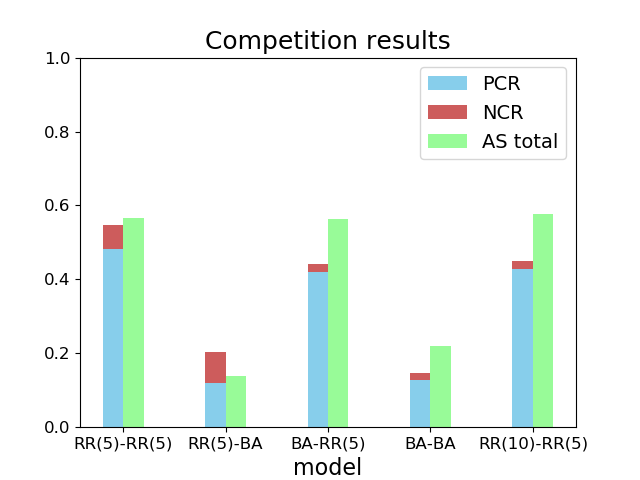
\includegraphics[width=\hsize]{FIG6.png}
	\caption{Comparison of Networks with different internal degrees(\textit{RR(n)-RR(m)}: layer A has random regular network with $n$ internal edges, layer B has random regular network with $m$ internal edges)}
	\label{Fig6}
\end{figure}
Next, the interconnected networks are simulated with different internal degrees in order to define and evaluate the influence of internal degrees. The number of internal degrees on each node is changed to $2$ or $5$.

Fig.~\ref{Fig6} shows the simulation result with changing the number of internal edges. \textit{RR(5)-RR(2)} has the most \textit{PCR}. \textit{RR(2)-RR(5)} has the most \textit{NCR}. When the number of internal edges in layer A are more than layer B, it has more efficient positive consensus. Inversely, when the number of internal edges in layer B are more than layer A, it has more efficient negative consensus, relatively. In other words, The number of edges on layer A has the tendency to keep positive state. The number of edges on layer B has the tendency to keep negative state. The number of internal edges have the influence on consensus result and a layer with more internal edges has the tendency to maintain its own state. In case of networks with same internal edges, \textit{RR(2)-RR(2)} has more \textit{PCR} and \textit{AS total} than \textit{RR(5)-RR(5)}. It can be analyzed that \textit{RR(5)-RR(5)} is hard to make consensus, because it has more internal edges to cause inner conflict. Also, \textit{RR(2)-RR(2)} has less \textit{NCR} than \textit{RR(5)-RR(5)}. It shows that the number of internal edges in layer B is more sensitive than layer A, because layer B dynamics are based on the number of degrees.   

\subsection{Competition on Networks with different structures}
So far, each layer of the interconnected network consisted of random regular network that has the same number of edges for each node. Now, the simulation would be implemented with changing network structures. 

\begin{figure}[!htb]
	\centering
	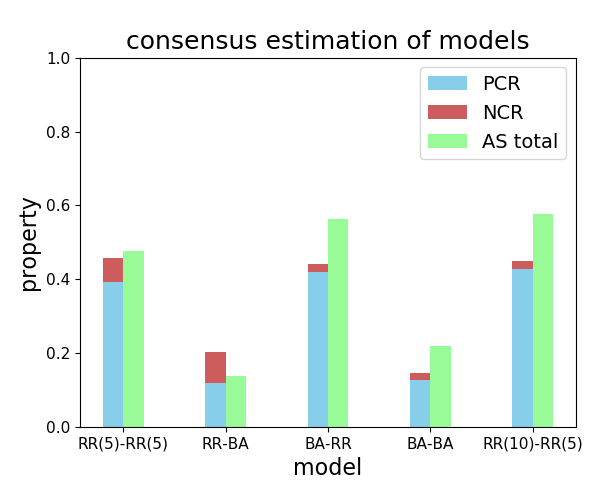
\includegraphics[width=\hsize]{FIG7.png}
	\caption{Comparison of Networks with different structures}
	\label{Fig7}
\end{figure}

To analyze and estimate interconnected network with different network structure, \textit{Barabasi-Albert network(BA)}\cite{barabasi1999} structure was applied for layer A. To evaluate the influence of network structure, 5 simulations were implemented with changing network structures. The BA network were applied for both layers or switched on each layer. And, because layer A of \textit{BA} network has total $10,215$ edges, \textit{RR(10)-RR(5)}, under the similar conditions such as the number of nodes and edges, was also simulated. The simulation results are shown as Fig.~\ref{Fig7}. The result properties of \textit{BA-RR} and \textit{RR(10)-RR(5)} are almost same. The gap of \textit{CR} is less than 0.007. The structure of network make no difference of consensus results. In case of \textit{BA-BA}, the \textit{CR} is the least ratio for consensus. \textit{`BA-BA'} structure has too many internal edges. Therefore, it is analyzed that it is hard to make consensus due to inner conflict on each layer. 

\section{Conclusion}
In this work, we have researched competing interconnected network dynamics. Layer A is a layer of social opinion and has positive states as an initial condition. It is influenced by opinion dynamics. Layer B is a network to represent a decision making layer, and has a negative state as an initial condition. It is influenced by the decision making dynamics. When these two layers were connected and interacted, it showed how their states were changed with switching $\gamma$ and $\beta$. The simulation result shows three final states, which are divided by the negative consensus, the positive consensus, and the coexistence according to $\gamma$ and $\beta$. We provided 4 competition results of different networks, which were derived from total $15$ simulations. Table.~\ref{tab1} shows simulation results of all models. 
\begin{table*}[!htb]
	\centering
	\caption{Consensus properties of Simulation Models}
	\label{tab1}
	\begin{center}
		\begin{tabular}{c|c|c|c|c|c|c|c|c} \hline\hline
			Div                    & A nodes& B nodes & A edges & B edges & AS total  & PCR    & NCR    & CR       \\ \hline \hline
			/RR(5)-RR(5)(30steps)   & 2,048  & 2,048   & 5,120   & 5,120   & 0.4760    & 0.3920 & 0.0660 & 0.4581   \\ \hline
			RR(5)-RR(5)(100steps)  & 2,048  & 2,048   & 5,120   & 5,120   & 0.5658    & 0.4828 & 0.0637 & 0.5466   \\ \hline
			RR-BA             	   & 2,048 	& 2,048   & 5,120   & 10,215  & 0.1397    & 0.1208 & 0.0839 & 0.2046   \\ \hline 
			BA-RR             	   & 2,048 	& 2,048   & 10,215  & 5,120   & 0.5622    & 0.4206 & 0.0220 & 0.4426   \\ \hline
			BA-BA             	   & 2,048 	& 2,048   & 10,215  & 10,215  & 0.2197    & 0.1273 & 0.0190 & 0.1463   \\ \hline
			RR(10)-RR(5)      	   & 2,048 	& 2,048   & 10,240  & 5,120   & 0.5776    & 0.4289 & 0.0220 & 0.4509   \\ \hline
			RR(2)-RR(2)            & 2,048 	& 2,048   & 2,048   & 2,048   & 0.7115    & 0.6377 & 0.0173 & 0.6550   \\ \hline 
			RR(2)-RR(5)            & 2,048 	& 2,048   & 2,048   & 5,120   & 0.0643    & 0.2272 & 0.1975 & 0.4247   \\ \hline 
			RR(5)-RR(2)            & 2,048 	& 2,048   & 5,120   & 2,048   & 0.8811    & 0.9060 & 0.0303 & 0.9363   \\ \hline
			Leader Model(2)        & 2,048 	& 1,024   & 5,120   & 2,560   & 0.6329    & 0.5725 & 0.0750 & 0.6475   \\ \hline    
			Leader Model(4)        & 2,048 	&  512    & 5,120   & 1,280   & 0.6951    & 0.6669 & 0.0781 & 0.7450   \\ \hline
			Leader Model(8)        & 2,048 	&  256    & 5,120   & 640     & 0.6768    & 0.6788 & 0.0856 & 0.7644   \\ \hline
			Leader Model(16)       & 2,048 	&  128    & 5,120   & 320     & 0.6350    & 0.6613 & 0.0988 & 0.7600   \\ \hline
			Leader Model(32)       & 2,048 	&   64    & 5,120   & 160     & 0.5753    & 0.6119 & 0.1056 & 0.7175   \\ \hline
			Leader Model(64)       & 2,048 	&   32    & 5,120   & 80      & 0.5064    & 0.5581 & 0.1106 & 0.6688   \\ \hline  \hline
		\end{tabular}
	\end{center}
\end{table*} 

Consensus and network state of each model are estimated with these simulation properties, such as \textit{AS total}, \textit{PCR}, \textit{NCR}, and \textit{CR}. Through comparison and analysis of these properties, we provide three conditions that increase the likelihood of consensus with social opinion.

Firstly, when the interconnected dynamics steps are increased with enough reinforcement($\beta$) above critical point, there is a high possibility of consensus with social opinion. Secondly, interconnected networks with leader help to make consensus. Leader Model were designed by reducing the nodes of decision-making layer at certain rate and increasing the external edges. The simulation results show  Leader Model have more consensus part than a leaderless model. Also, it is found out that there is the efficient number of leader for making consensus. Thirdly, social opinion layer requires more internal edges than opposite layer in order to make positive consensus. When the networks were simulated with different internal edges, the result shows that a layer with more internal edges has more tendency to keep its own states. In addition, it provides that too many internal edges can cause inner conflict, and that make it hard to have consensus state.  

More research will be needed to make generalized model and to be applied to real social networks. We think this research can contribute to providing the analysis tool of competing social networks such as the legalization or social decision-making system. Also, it could help to solve the social conflict by making consensus of two layer. As the future work, it would be very interesting to make the generalized model for competing interconnected network and find the key nodes and edges of interconnected network.

\begin{thebibliography}{0}
\bibitem{bianconi2018}
G. Bianconi, \textit{Multilayer Networks: Structure and Function}, Oxford University Press, 2018.

\bibitem{domenico2013}
M. De Domenico et al, \textit{Mathematical Formulation of Multilayer Networks}, Physical Review X 3, 041022, 2013.

\bibitem{tomasini2015}
Marcello Tomasini, \textit{An Introduction to Multilayer Networks}, 10.13140/RG.2.2.16830.18243, 2015.

\bibitem{kimsangwoo2012}
Kim Sangwoo, \textit{Structure and dynamics of complex networks}, Yonsei Univ, 2012.

\bibitem{newman2010}
M. E. J. Newman, \textit{Networks: An Introduction}, Oxford University Press, 2010.
	
\bibitem{boccaletti2014}
S. Boccaletti et al, \textit{The structure and dynamics of multilayer networks}, Physics Reports 544, 2014.	

\bibitem{hua2014}
Hua Jun, Lin Wang, Xiaofan Wang, \textit{An information diffusion model based on individual characteristics}, 33rd Chinese Control Conference (CCC), 2014.

\bibitem{shenyu2018}
Shenyu Zhou,  Shuyang Shi, Lin Wang, \textit{Immunizations of Interacting Diseases}, 37rd Chinese Control Conference (CCC), 2018.
	
\bibitem{mikko2013}
Mikko Kivela et al, \textit{Multilayer Networks}, J. Complex Networks Volume 2. DOI : 10.1093/comnet/cnu016, 2013.	
	
\bibitem{huberman2004}
Wu F. and Huberman B.A, \textit{Social structure and opinion formation}, arXiv.org:cond-mat/0407252v3, 2004	


	
	
	
	
	
\bibitem{amato2017}
R Amato et al, \textit{Opinion competition dynamics on multiplex networks}, New Journal of Physics volume 19, 2017

\bibitem{quattrociocchi2014}
Walter Quattrociocchi et al, \textit{Opinion dynamics on interacting networks : media competition and social influence}, Scientific Reports:Complex networks Statistical Physics, 2014

\bibitem{haibo2017}
Haibo Hu, \textit{Competing opinion diffusion on social networks}, Royal Society Open Science volume 4, 2017




\bibitem{redner2017}
Sidney Redner, \textit{Dynamics of Voter Models on Simple and Complex Networks}, Physics and Society(physics.soc-ph), 2017





\bibitem{smyrnakis2019}
Michalis Smyrnakis et al, \textit{An evolutionary game perspective on quantised consensus in opinion dynamics}, PLoS ONE 14(1):e0209212, 2019





\bibitem{danziger2019}
Danziger, Michael M. et al, \textit{Dynamic interdependence and competition in multilayer networks}, Nature Physics Volume 15. pp.178-185, 2019.

\bibitem{namkhanhvu2017}
Nam Khanh Vu, \textit{Robustness of Interconnected Complex Networks with Directed Dependency}, Yonsei University Department of Computer Science, 2017.

\bibitem{laguna2004}
M. F. Laguna et al, \textit{The dynamics of opinion in hierarchical organizations}, arXiv.org:nlin/0404024, 2004 

\bibitem{masuda2015}
Naoki Masuda, \textit{Opinion control in complex networks}, New Journal of Physics, Volume 17, 2015.

\bibitem{zuev2012}
Zuev A S and Fedyanin, 
\textit{Models of opinion control for agents in social networks}, Automation and Remote Control Volume 73 Issue 10, pp.1753–1764, 2012 








\bibitem{alvarez2016}
Alvarez Zuzek et al, \textit{Interacting Social Processes on Interconnected Network}, PLoS ONE. 11. 10.1371/journal.pone.0163593, 2016.

\bibitem{gomez2015}
Gomez Gardenes J. et al, \textit{Layer-layer competition in multiplex complex network}, Phil. Trans. R. Soc. A 373:20150117, 2015

\bibitem{diep2017}
H.T. Diep et al, \textit{Dynamics of two-group conflicts: A statistical physics model}, Physica A: Statistical Mechanics and its Applications Volume 467. pp.183 - 199, 2017.

\bibitem{rocca2014}
C. E. La Rocca et al, \textit{The influence of persuasion in opinion formation and polarization}, Europhys. Lett. 106, 40004, pp.1-2, 2014.

\bibitem{velasquez2018}
F. Vel{\'a}zquez et al,\textit{Opinion dynamics in two dimensions: domain coarsening leads to stable bi-polarization and anomalous scaling exponents}, Physics and Society(physics.soc-ph), 2018. 








\bibitem{abrams2003}
M Abrams et al, \textit{Modelling the dynamics of language death}, Nature.424.900. DOI : 10.1038/424900a, 2003.

\bibitem{vazquez2010}
 F. V{\'a}zquez et al, \textit{Agent based models of language competition: macroscopic descriptions and order–disorder transitions}, Journal of Statistical Mechanics: Theory and Experiment P04007, 2010.

\bibitem{bela2001}
 Bela Bollobas, \textit{Random Graphs}, 2nd edition, Cambridge University Press, section 2.4: Random Regular Graphs, 2001.

\bibitem{barabasi1999}
Barabasi A. L., Albert R, \textit{Emergence of Scaling in Random Networks}, Science 286, 509, DOI: 10.1126/science.286.5439.509, 1999.



\end{thebibliography}

\end{document}



































